% ---------------------------------------------------------------------------
\section{Robustness: GRPO, Group Size, Many Answers, Adam}
\label{sec:robust}

All discussions in the main text use one training setup: REINFORCE with $K=3$, binary answers and plain SGD. Here we vary each of these choices, still in the toy model, to check that the law of \cref{sec:theory} is not an artifact of the defaults.

\begin{figure}[t]
\centering
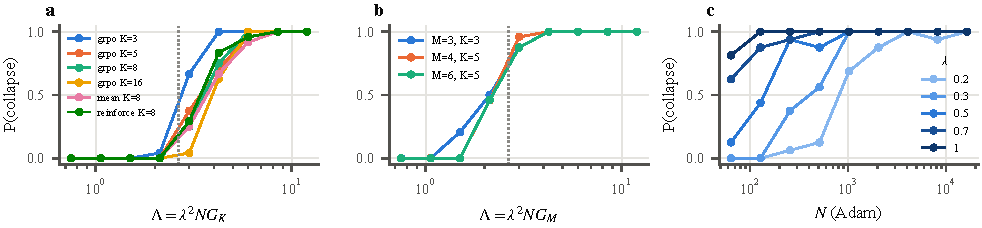
\includegraphics[width=\textwidth]{../figures/fig_robust.pdf}
\caption{\textbf{Robustness.} (a)~GRPO and REINFORCE for $K\in\{3,5,8,16\}$ against $\Lambda=\lambda^2NG_K$, where $G_K$ (\cref{sec:race}) is computed from the exact $K$-sample drift $F_K$ (\cref{sec:single}). (b)~$M$-answer softmax policies against $\Lambda=\lambda^2NG_M$. (c)~Adam: probability of collapse against $N$ for several couplings.}
\label{fig:robust}
\end{figure}

\begin{table}[h]
\caption{Edge of the unstable window $z^\star_K$ (where $F_K'=0$) and the amplification factor $G_K(0.5)=\ln[F^\star_K/F_K(0.5)]$ for different estimators and group sizes $K$ (binary answers). Computed exactly by enumeration.}
\label{tab:window}
\centering\small
\begin{tabular}{lccccc}
\toprule
 & $K=3$ & $4$ & $5$ & $8$ & $16$ \\
\midrule
\multicolumn{6}{l}{\emph{REINFORCE:} $z^\star_K$} \\
 & 1.317 & 1.274 & 1.187 & 1.088 & 0.894 \\
\multicolumn{6}{l}{\emph{GRPO (std-normalized):} $z^\star_K$} \\
 & 1.317 & 1.317 & 1.213 & 1.172 & 1.006 \\
\midrule
\multicolumn{6}{l}{\emph{REINFORCE:} $G_K(0.5)$} \\
 & 0.514 & 0.484 & 0.426 & 0.353 & 0.202 \\
\multicolumn{6}{l}{\emph{GRPO:} $G_K(0.5)$} \\
 & 0.514 & 0.514 & 0.443 & 0.408 & 0.258 \\
\bottomrule
\end{tabular}
\end{table}

\paragraph{GRPO and group size.}
For $K=3$, GRPO's drift is exactly $\sqrt2F$ (\cref{sec:single}). The constant factor cancels in $G$, so $G_3(0.5)=0.514$ for both estimators (\cref{tab:window}), and the theory predicts the same $N_c$.
The simulations agree: the logistic fit to the GRPO $K=3$ curve in \cref{fig:robust}a gives $N_c=548$, against $N_c=536$ for REINFORCE at the same $\lambda=0.1$ and $a=0.5$ (\cref{fig:scaling}c).
Larger groups have smaller $G_K$ (\cref{tab:window}), so the theory predicts larger $N_c$. The fitted values rise to $793$, $876$ and $1557$ for $K=5,8,16$ (\cref{fig:robust}a), in the order predicted by $G_K$.
Computing $\Lambda_c=\lambda^2N_cG_K$ from these fits, the critical amplification drifts mildly upward with $K$ ($\Lambda_c=2.8\to4.0$), consistent with the smaller gradient noise and hence smaller seed $\delta$ of larger groups.
The mean baseline and REINFORCE at $K=8$, also shown in \cref{fig:robust}a, give $\Lambda_c=3.8$ and $3.5$, within this band.

\paragraph{Many answers.}
Next we replace binary answers by $M$-answer softmax policies, as in the theory of \cref{sec:general}.
With $M\in\{3,4,6\}$ answers, softmax logits and a shared bias \emph{vector}, the collapsed state has every problem giving the same answer, and accuracy drops to $1/M$.
Using the eigenvalue-based $G_M$ of \cref{sec:general}, computed by exact enumeration (\cref{app:multi}), the transitions fall at $\Lambda_c=2.1$--$2.2$ (\cref{fig:robust}b), slightly below the binary value. This is consistent with $M-1$ noisy shared directions seeding the instability.

\paragraph{Adam.}
The last change is the optimizer. Unlike the changes above, it alters the rates in the theory itself, so we first rederive the scaling.
Adam \citep{kingma2015adam} normalizes each coordinate by its own gradient scale, which changes both rates in the race.
The shared parameter sees a gradient dominated by noise of scale $\lambda\sigma/\sqrt B$, so its signal-to-noise-normalized drift makes the shared mode grow at a rate $\propto\lambda\langle F'\rangle$ rather than $\lambda^2\langle F'\rangle$.
A problem-specific coordinate is updated only on a fraction $B/N$ of steps, so its normalized step grows like $\sqrt{N/B}$ per epoch.
The ratio gives $\Lambda_{\mathrm{Adam}}\propto\lambda\sqrt N\,G$, and therefore the \emph{same} scaling $N_c\propto\lambda^{-2}$ with a different constant.
Simulations agree (\cref{fig:robust}c). For $\lambda\in\{0.2,0.3,0.5\}$ we find $N_c=899,378,136$, so $\lambda^2N_c=34$--$36$ is constant (fitted slope $-2.06$). With our hyperparameters this constant is about $9\times$ the SGD value at the same coupling ($\lambda^2N_c\approx4.0$ at $\lambda=0.2$, \cref{fig:scaling}c), so Adam is more tolerant, but the law is unchanged.
(For $\lambda\ge0.7$, $N_c$ falls below the smallest size we simulate.)
